\documentclass{article}
\usepackage{tikz}
\usepackage{amsmath,amssymb}
\usetikzlibrary{shapes, arrows, chains}
\tikzstyle{line} = [draw, -latex']
\begin{document}
	
\title{ExaGEP Plan of Work}

\author{G.~A.}

\maketitle

\section{Representation of Circuits}

\begin{figure}[h]\centering{%
	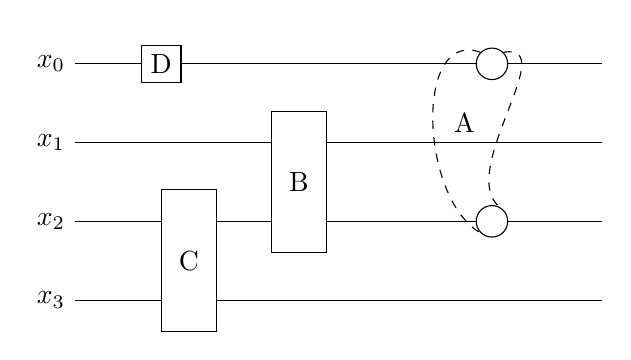
\begin{tikzpicture}
		\def\yl{-1}
		\def\xl{7}
		\node (x0) at (0,0) {$x_0$};
		\node (x1) at (0, \yl) {$x_1$};
		\node (x2) at (0, 2*\yl) {$x_2$};
		\node (x3) at (0, 3*\yl) {$x_3$};
		\coordinate (l0) at (\xl, 0);
		\coordinate (l1) at (\xl, \yl);
		\coordinate (l2) at (\xl, 2*\yl);
		\coordinate (l3) at (\xl, 3*\yl);
		\draw (x0) -- (l0);
		\draw (x1) -- (l1);
		\draw (x2) -- (l2);
		\draw (x3) -- (l3);
		\node[rectangle,draw=black,fill=white] at (0.2*\xl, 0) {D};
		\draw[fill=white] (0.4*\xl, 0.6*\yl) -- (0.5*\xl, 0.6*\yl) -- (0.5*\xl, 2.4*\yl) -- (0.4*\xl, 2.4*\yl) -- cycle;
		\node at (0.45*\xl, 1.5*\yl) {B};
		\draw[fill=white] (0.2*\xl, 1.6*\yl) -- (0.3*\xl, 1.6*\yl) -- (0.3*\xl, 3.4*\yl) -- (0.2*\xl, 3.4*\yl) -- cycle;
		\node at (0.25*\xl, 2.5*\yl) {C};
		\node[circle, draw=black, minimum size=0.4cm, fill=white] (A0) at (0.8*\xl, 0) {};
		\node[circle, draw=black, minimum size=0.4cm, fill=white] (A1) at (0.8*\xl, 2*\yl) {};
		\draw[dashed] (A0.north west) to[out=160, in=150] (A1.south west);
		\draw[dashed] (A0.north east) to[out=10, in=150] (A1.north east);
		\node at (0.75*\xl, 0.75*\yl) {A};
	\end{tikzpicture}}
	\caption{\label{fig:circuit}
		An example of a 4-bit quantum circuit with gates A, B, C, and D in order
		to explain the circuit encoding in genetic expression programming.}
\end{figure}
\begin{figure}[h]\centering{%
	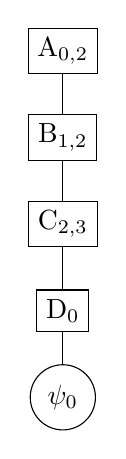
\begin{tikzpicture}
		\def\yn{1.1}
		\def\xn{2.5}
		\node[circle, draw=black] (x0) at (0, 0) {$\psi_0$};
		\node[rectangle,draw=black,fill=white] (D) at (0, \yn) {D$_0$};
		\node[rectangle,draw=black,fill=white] (C) at (0, 2*\yn) {C$_{2,3}$};
		\node[rectangle,draw=black,fill=white] (B) at (0, 3*\yn) {B$_{1,2}$};
		\node[rectangle,draw=black,fill=white] (A) at (0, 4*\yn) {A$_{0,2}$};
		\draw (x0) -- (D);	
		\draw (D) -- (C);
		\draw (C) -- (B);
		\draw (B) -- (A);
	\end{tikzpicture}}
\caption{Representation of the previous figure's quantum circuit in Genetic Expression Programming.
The ``primitives'' or gates are D$_{0}$, C$_{2, 3}$, B$_{1, 2}$, and A$_{0, 2}$.
Every primitive takes one input and produces one output.
The final output is A$_{0,2}$B$_{1,2}$C$_{2,3}$D$_0\psi_0$.}
\end{figure}

The 4-bit quantum circuit in Fig.~\ref{fig:circuit} needs to be represented in genetic expression programming.
We define the Hilbert space $\mathcal{H}=\mathbb{C}^{2^N}$, with its usual inner product.
so that the inputs are in $\mathcal{H}$.

\subsection{Gates}
Gates are the GEP primitives, and are functions of $\mathcal{H}$ into $\mathcal{H}$.
The multiplicity of a one-bit gate (like the Hadamard gate) is $N$;
the multiplicity of a two-bit gate (like the CNOT gate) is $N(N-1)$;
the multiplicity of a three-bit gate (like the CCNOT gate) is $N^3-3N(N-1)-N$.

\subsection{Encoding as a String}
The gene for Figure 2 is encoded by the string A$_{0,2}$B$_{1,2}$C$_{2,3}$D$_0\psi_0$.

\section{Optimization Procedure}
Given a state $|\psi^{\textrm{known}}\rangle$, we want to find a quantum
circuit $\mathcal{C}_{\textrm{unknown}}$ that generates it for an initial state $|\psi_0\rangle$,
that is, that satisfies 
\begin{equation}
	|\psi^{\textrm{known}}\rangle=\mathcal{C}_{\textrm{unknown}}|\psi_0\rangle.
\end{equation}
The genetic expression programming procedure to find such a circuit is as follows.

\begin{enumerate}
	\item Start with an original population of $M=100$ circuits generated randomly.
	\item Start with a pure state ket of length $N$: $|\psi_0\rangle\equiv|x_0, x_1, \ldots, x_{N-1}\rangle$.
	\item By genetic expression programming mutations and combinations of the original 
	population created in step 1, generate $M'=200$ new circuits
	$\{\mathcal{C}(\varphi)\}_{0\le j<M}$. These circuits may depend on
	$K$ continuous variables
	$\varphi\equiv\{\varphi_k\}_{0\le k<K}$. To understand why this is so, consider that the rotation gate
	may depend on the angle of rotation, and, in general, gates may depend on arbitrary parameters that
	we collectively call $\varphi$.
	\item For every circuit $j$, define the $\varphi-$dependent ket $\psi_j(\varphi)\equiv\mathcal{C}_j(\varphi)|\psi_0\rangle$.
	\item For every circuit $j$, define the pre-fitness $P_j$ function by
	\begin{equation}
		P_j(\varphi) \equiv |\langle \psi^{\textrm{known}} | \psi_j(\varphi)\rangle|^2
	\end{equation}
	and find the $\varphi$ where the maximum occurs; let's call it $\varphi_{\textrm{max}}$.
	\item For every circuit $j$, calculate its fitness $F_j \equiv P_j(\varphi_{\textrm{max}})$.
	\item Eliminate the $M'-M=100$ circuits with less fitness and keep the others.
	\item Go to step 3. 
\end{enumerate}
\end{document}

